\chapter{Gemination} \label{Gemination}


In this chapter, I will introduce and clarify the key terminology and notions necessary to understand the theoretical implications of this book. I will discuss different types of {geminates} and thereby show how \isi{gemination} is a phonological as well as a morphological phenomenon. I will also explain the important role of phonetics in investigating \isi{gemination}. After clarifying some general notions on \isi{gemination}, I will concentrate on \isi{gemination} in English by reviewing assumptions and previous research. 

\section{Geminates} \label{what is gemination}

Geminates are taken to be double consonants which are articulated with a particularly long duration (e.g. \citealt{Hartmann.1972, Catford.1988, Trask.1996, Matthews.1997, Crystal.2008,Davis.2011, Galea.2016}). Lexical (or ``true'') \is{lexical gemination}{geminates} denote a phonemic difference, i.e. they make up minimal pairs with their singleton counterparts such as in the Japanese words  \textit{kona} ‘powder’ versus \textit{konna} ‘such'. A second type of {geminate} are double consonants arising across a morphological boundary from the concatenation of two morphemes, such as in the English prefixed word \textit{unnatural} or the compound \textit{fun name}. For this type of {geminates} various labels are found in the literature, among them \textit{fake  {geminates} }(for example used by \citealt{Hayes.1986b}; \citealt{Oh.2012} and \citealt{Kotzor.2016}), \textit{derived geminates} (for example used by \citealt{Kubozono.2017b}), \textit{concatenated {geminates}} (for example used by \citealt{Ridouane.2010}) and \textit{surface {geminates}} (for example used by \citealt{Lahiri.1988, Galea.2016}). I will refer to them as \is{morphological gemination}\textit{morphological {geminates}}.


The main feature of {geminates}, distinguishing them from singletons, is their longer duration. But what is the durational difference between {geminates} and singletons? Acoustic research has shown that there is no universal answer to this question. The singleton-{geminate} ratio \is{singleton-geminate ratio} depends on various factors, such as the language in which the geminate occurs, the type of segment the geminate consists of and the {geminate's} position. With regard to cross-linguistic differences a review of empirical work on the topic reveals quite a big range of singleton-{geminate} ratios between languages.  Stop {geminates} in word-medial position are, for example, found to range from 1:1.5 in Madurese (\citealt{Cohn.1999}) to 1:2.9 in Turkish (\citealt{Lahiri.1988}) (see also \citealt[38 f.]{Dmitrieva.2017} for discussion of language-specific differences). 
Furthermore, durational differences heavily depend on the type of segment involved. For instance, \cite{Aoyama.2006} find that for Guinaang Bontok the highest ratios, i.e. the longest {geminates}, can be found with nasals (ratios between 1:1.72 and 1:2.15), followed by lateral approximants (ratio: 1:2.0), stops (ratios between 1:1.81 and 1:1.90), approximants (ratios between 1:1.56 and 1:1.69) and fricatives (ratio for [s]: 1:1.56). The lowest ratio is found for glides (ratio: 1:1.39). Similarly, for Italian,  \cite{Payne.2005} finds the longest \is{lexical gemination}{geminates} with nasals and laterals (ratio for nasals: 1:2.1, ratio for laterals: 1:2.3) and the shortest with fricatives (ratio: 1:1.5). 
 The influence of position is yet unclear and seems to depend on the language investigated (see \citealt[chapter 3]{Galea.2016} and \citealt[36 f.]{Dmitrieva.2017} for a discussion of cross-linguistic {gemination} in different positions). While \cite{Ridouane.2010}, for example, finds that word-final {geminates} are longer than word-medial {geminates} in Tashlhiyt Berber, \cite{Kraehenmann.2001} finds the opposite for Swiss German. For Maltese, \cite{Galea.2016} finds, similarly to Kraehenmann, word-medial {geminates} to be longer than word-final {geminates}. Studies on word-initial and word-final {geminates} are, however, quite rare. One reason for the low number of investigations on the topic might be that most {geminates} occur in  word-medial position (\citealt[34]{Dmitrieva.2017}; \citealt[11]{Topintzi.2017}). Whether there is a systematic difference in duration between {geminates} in different positions is to be determined in further research.
 

In addition to \is{absolute duration}duration, there are some other possible acoustic correlates of \is{lexical gemination}{gemination} discussed in the literature. In a study on Tashlhiyt Berber, \cite{Ridouane.2010}, for example, shows  that {lexical geminates} differ in their  amplitude, as well as in the duration of their preceding vowel from their singleton counterparts. Geminates feature a higher amplitude and are preceded by a shorter vowel than singletons. While amplitudinal features of {geminates} are not well researched,  the shortening of a geminate-preceding vowel was also found in other studies, such as in \cite{Lahiri.1988} for Bengali, in \cite{Cohn.1999} for Buginese, Madurese and Toba Batak and in  \cite{Galea.2016} for Maltese (see also \citealt{Maddieson.1985} for discussion). However, there are also studies which did not find the duration of the preceding vowel to be affected by {gemination} (cf. for example \citealt{Lahiri.1988} on Turkish, \citealt{Ham.2001} on Hungarian, see also \citealt[6]{Ridouane.2010} for a review of temporal acoustic attributes of {gemination} in different languages).

To summarize, even though there is evidence that in some languages \is{lexical gemination}{geminates} might affect the duration of their preceding vowel, as well as other acoustic properties, such as amplitude, the core feature of {geminates} is their internal, longer duration \is{absolute duration}. Geminates are significantly longer than their singleton counterpart. Importantly, the \isi{singleton-geminate ratio} is not universal and may vary depending on language, {geminate} position and the segmental features of the segment.



\section{Morphological geminates}\label{Morphological Gemination}

As mentioned in the previous section, there are two different types of geminates: lexical and \is{morphological gemination} morphological geminates. In English, the language under investigation in this book, \is{lexical gemination}{lexical geminates} do not exist. However, English has \is{morphological gemination} morphological geminates. Two adjacent identical consonants may either emerge word-internally through \isi{affixation} (e.g. \textit{unnatural}), or across a word boundary in compounding (e.g. \textit{book case}) and in phrases (e.g. \textit{The man naps.}). In this book, I will concentrate on \is{morphological gemination}{gemination} in English \isi{affixation}. Affixational geminates emerge in prefixed words when the final segment of a prefix and the first segment of the base are identical. In suffixed words a {morphological geminate} emerges when the first segment of the suffix and the last segment of the base are identical. Examples of geminates with prefixed and suffixed English words are given in (\ref{example gemination 1}) and (\ref{example gemination 2}). Note that while in most cases the phonological double consonant is represented by an orthographic double, there are also some words in which the two identical consonants are interrupted by  an additional character (e.g. \textit{unknown, solely}).

\begin{exe} 
	\ex \label{example gemination 1} \textit{unnatural, unknown, innumerous, immortal, dissatisfied}
	\ex \label{example gemination 2}\textit{really, solely, cleanness, soulless}
\end{exe}

While the durational features of \is{lexical gemination}{lexical geminates} are clear in the sense that they are significantly longer than their singleton counterparts, facts are less clear with \is{morphological gemination} morphological geminates. Since \is{morphological gemination} morphological geminates do not denote a phonemic difference, there are essentially two possibilities for their \isi{phonetic realization}: preservation and \isi{reduction}. If the two consonants are preserved, I will speak of \isi{gemination}. If the two consonants are reduced, I will speak of \isi{degemination}. 
In case of preservation one should expect a significant durational difference between a double consonant and a singleton, with the double consonant being longer.	
In the case of \isi{reduction}, i.e. \isi{degemination}, two options are possible. The first is categorical in nature: one of the two underlying consonants would be deleted, to the effect that there would be no durational difference between a singleton and the degeminated double consonant.
Another option is that \isi{degemination} is a gradient phenomenon. Under this view the potential \isi{reduction} of two identical consonants straddling a morphological boundary is gradual and could depend on word-specific properties, for example the \isi{morphological decomposability} of the word in question. 
While most theoretical approaches expect \isi{gemination} to be categorical, the question is yet unanswered and needs to be addressed empirically (see \sectref{decomposability} for further discussion).

% generally morph. geminates
In general, \is{morphological gemination} morphological geminates are investigated less than \is{lexical gemination} lexical geminates, and only a few studies are available which empirically investigated the matter. One prominent idea tested in the available studies is whether there is a difference in the realization of geminates with different types of morphological boundaries.
 For example, \cite{Bergmann.2017} conducted an experimental study on {gemination} in German nominal compounds (e.g. \textit{Schifffenster}, Eng. ‘{ship window}') and  particle verbs (e.g. \textit{auffallen}, Eng.  ‘{notice}'). She found that both constructions geminate and that the \isi{degree of gemination}, i.e. the duration of the double consonant, depends on \isi{accentuation}, as well as lexical \isi{frequency}. Duration is enhanced with low \isi{frequency} words, as well as when a word bears sentence \is{accentuation} accent. The study thus shows that the realization of \is{morphological gemination} morphological geminates is influenced by prosodic, as well as lexical factors. Bergmann's results do, however, not support the idea that the realization of geminates is influenced by the type of morphological boundaries across which they occur. In her study there was no difference in the realization of geminates across compound-internal boundaries and word-internal geminates in particle words.


\cite{Ridouane.2010} found similar results for the influence of different morphological boundaries on geminate duration in Tashlhiyt Berber. He compared the phonetic correlates of \isi{gemination} in word-initial \is{lexical gemination} lexical geminates with the ones in word-initial \is{morphological gemination} morphological geminates. The \is{morphological gemination} morphological geminates display the same durational differences to singletons as the \is{lexical gemination} lexical geminates. In other words, with regard to \is{absolute duration}duration, morphological and \is{lexical gemination} lexical geminates are alike. However, while \is{lexical gemination} lexical geminates also display shorter preceding vowel durations and higher amplitudes than singletons, these secondary cues of \isi{gemination} were not found for \is{morphological gemination} morphological geminates. These results fit in with Bergmann's, as both studies do not find durational differences depending on the morphological boundary of the geminate. However, in contrast to Bergmann, Ridouane found additional phonetic differences between geminates with different {boundary strengths}, suggesting that \isi{boundary strength} might indeed play a role in {gemination}. 
\cite{Ridouane.2010} interprets the acoustic differences between lexical and \is{morphological gemination} morphological geminates as arising from differences in the \isi{underlying representation} of the two different types of geminates.  According to him the representations of \is{lexical gemination} lexical geminates are ``stronger'' than the ones of \is{morphological gemination} morphological geminates. Therefore, \is{lexical gemination} lexical geminates feature, in contrast to \is{morphological gemination} morphological geminates, enhancing correlates (such as higher amplitudes and shorter preceding vowel durations)  \textendash a suggestion which I will discuss in more detail in \sectref{Phonological representation of geminates}. 

A study conducted on Maltese word-initial geminates by \cite{Galea.2014} also supports the idea that lexical and \is{morphological gemination} morphological geminates differ in their underlying structure and \isi{phonetic realization}. Galea et al. found shorter durations for \is{morphological gemination} morphological geminates than for \is{lexical gemination} lexical geminates. While the durational differences found do not fit in with \citeauthor{Ridouane.2010}'s (2010) results, the finding that \is{morphological gemination} morphological geminates generally differ from \is{lexical gemination} lexical geminates in their \isi{phonetic realization} fits in with \citeauthor{Ridouane.2010}'s idea of \is{lexical gemination} lexical geminates being ``stronger'' than \is{morphological gemination} morphological geminates. In contrast to \is{morphological gemination} morphological geminates they are not affected by weakening processes, such as phonetic \isi{reduction}. 

As discussed above, in contrast to the results by \cite{Ridouane.2010} and \cite{Galea.2014}, no difference was found between the different types of geminates in \cite{Bergmann.2017}, i.e. \cite{Bergmann.2017} did not find differences in the realization of word-internal geminates in particle words and word-boundary geminates in compounds. This opens up the question of whether differences only exist between the geminates of certain types of morphological boundaries, such as morphological vs. non-morphological. However, the three studies discussed deviate from each other in many respects, so that no firm conclusions can be drawn. First, the studies investigated geminates in different positions. While Bergmann looked at word-medial geminates, Ridouane and Galea et al. investigated word-initial geminates. Second, the three studies looked at different languages. As discussed in \sectref{what is gemination}, the realization of geminates differs between languages. Therefore, differences in results might be due to language-specific factors. A third potential cause for the deviating results might be that different types of segments were investigated. Further studies which systematically look at the influence of \isi{morphological boundary strength} on \isi{gemination} in different languages are needed to clarify the matter. It is especially necessary to address the question of whether only a binary distinction between morphological vs. \is{lexical gemination} lexical geminates exists, or whether different types of \is{morphological gemination} morphological geminates show differences.


For English six studies on \isi{morphological gemination} exist: \cite{Delattre.}, \citet{Kaye.2005}, \citet{Oh.2012}, \cite{Oh.2013}, \cite{Kotzor.2016} and \cite{BenHedia.2017}. While some insights about English geminates can be gleaned from these studies, due to methodological reasons, as well as sample size, many aspects of \isi{morphological gemination} in English remain unknown. I will discuss each study in detail in \sectref{Gemination in English}.\footnote{\cite{BenHedia.2017} is part of this book and will be discussed in chapter \ref{Corpus Studies}.} Before turning to \isi{morphological gemination} in English though, I will discuss the \isi{phonological representation} of geminates, particularly the representation of \is{morphological gemination} morphological geminates.



\section{Phonological representation of geminates } \label{Phonological representation of geminates}

The \isi{phonological representation} of geminates has been a topic of discussion for decades and  ``will remain an area of theoretical controversy in the foreseeable future'' \cite[22]{Davis.2011}. The main question of dispute is whether geminates should be represented as one or two underlying phonological segments. To understand why this question is raised, we need to take a look at the phonological properties of geminates. 

According to \cite{Hayes.1986b} \is{lexical gemination} lexical geminates are characterized by three phonological properties: ambiguity, integrity and inalterability. Ambiguity refers to the ambiguous phonological behavior of geminates. In some respects they behave as if they were two segments (e.g. their duration and their ambisyllabicity), and in some they behave as if they were one (e.g. one feature bundle). Integrity refers to the fact that geminates  cannot be split up by rules of epenthesis (see, for example,  \citealt{AbuSalim.,Kenstowicz.1994}).  Inalterability alludes to the {geminate's} resistance to undergo \is{phonological rule}{phonological rules} that are expected to apply to its singleton counterpart, such as for example spirantization (see, for example, \citealt {Kenstowicz.1994} and \citealt[chapter 5]{Kirchner.2001} for discussion). 

The \isi{phonological representation} of geminates should accommodate all three properties, i.e. capture that geminates are like two segments in some respects and like one in others. This already poses a challenge for phonological theory. The fact that geminates do not display universal behavior across languages complicates the matter further. For example, \cite{Kenstowicz.1994} notes that Icelandic geminates violate the inalterability aspect. When part of a consonant cluster, the first part of the geminate undergoes a \isi{phonological rule} which shifts its aspiration to the preceding segment, i.e. the geminate is altered.
 The variation in the phonological behavior of geminates across languages might suggest that there is no universal representation of geminates.  This view is for example taken by \cite{Ham.2001}, who suggests that representations are language-specific and may even differ within one language depending on geminate position in the word.
 
Interestingly, the discussion about the representation of geminates mainly revolves around \is{lexical gemination} lexical geminates and not around morphological  geminates. One reason is that, according to the literature, \is{morphological gemination} morphological geminates behave differently than \is{lexical gemination} lexical geminates. They allow for epenthesis, i.e. are not characterized by integrity, and  undergo phonological alternations, i.e. are alterable (see also \citealt{Kenstowicz.1994,Kirchner.2001} and \citealt{Ridouane.2010} for discussion). Therefore, one can state that \is{morphological gemination} morphological geminates are not characterized by  the same three phonological properties as \is{lexical gemination} lexical geminates. 
As discussed above, there is also empirical evidence for different underlying representations of lexical and \is{morphological gemination} morphological geminates (cf. \citealt{Ridouane.2010,Galea.2014}). While for \is{lexical gemination} lexical geminates there are arguments for a single \isi{underlying representation} (such as their inalterability and integrity), \is{morphological gemination} morphological geminates behave like two adjacent segments and are therefore commonly represented by two segments. This view ties in with \citeauthor{Ridouane.2010}'s argument of \is{lexical gemination} lexical geminates having a stronger representation than morphological ones.

The two most-discussed ways of representing geminates are the {autosegmental representation} (see, for example, \citealt{Leben.1980,Hayes.1986b,Levin.1985,Ridouane.2010}) and the {moraic representation}  (see, for example, \citealt{Hayes.1989,Davis.2014,Topintzi.2008}). 
The {autosegmental representation}, first proposed by \cite{Leben.1980}, uses two separate tiers to capture the ambiguous structure of \is{lexical gemination} lexical geminates \textendash the skeletal tier\footnote{The skeletal tier is also referred to as \textit{CV-tier} (cf., for example, \citealt{Hayes.1986b, Ridouane.2010,Ridouane.2017}), \textit{X-tier} (cf., for example, \citealt{Levin.1985}) or  \textit{length-tier} (cf., for example, \citealt{Vago.2011}). The different labels mirror differences in the approaches which are not relevant for the current book and will therefore not be discussed here.}
and the segmental tier. While the skeletal tier represents the prosody of a structure, the segmental tier represents its segments. 

\begin{figure}[h]
	\centering	
	
	\begin{tabularx}{.8\linewidth}{YYY}
		
		&		lexical			 & 		 morphological \\
		
		singleton	&			  geminate	 & 			  geminate\\		
		\\

		\begin{tikzpicture}[grow'=up]
		\Tree [.C C ] 					
		\end{tikzpicture}												&
		
		
		\begin{tikzpicture}[grow'=up]
		\Tree  [.C C C ];
		\end{tikzpicture}			
		&
		
		\begin{tikzpicture}[grow'=up]
		\Tree  [.C C ]
		\end{tikzpicture}
		\begin{tikzpicture}[grow'=up]
		\Tree  [.C C ]
		\end{tikzpicture}		
		
	\end{tabularx}
	
	\caption{Autosegmental representation of geminates}
	 \label{fig:Autosegmental representation of geminates} 

\end{figure}

\figref{fig:Autosegmental representation of geminates} shows the autosegmental representations of singletons, \is{lexical gemination} lexical geminates and \is{morphological gemination} morphological geminates (for similar analyses see, for example,  \citealt[413]{Kenstowicz.1994}, \citealt[26 f.]{Gussmann.2002} and \citealt[62]{Ridouane.2010}). The upper tier shows the skeletal tier and the lower one the segmental. While singletons only take one slot at both levels, \is{lexical gemination} lexical geminates occupy one slot at the segmental tier and two slots on the skeletal tier. The two prosodic slots account for the long duration of the geminate, as well as for its ambisyllabicity. The single slot on the segmental tier represents the {geminate's} inalterability and integrity. Since \is{morphological gemination} morphological geminates differ from \is{lexical gemination} lexical geminates in terms of their integrity and inalteribility, they take two slots on both tiers. This also mirrors their derivational nature, which naturally entails that a {morphological geminate} is made of two concatenated identical segments.


Differently from the autosegmental approach, the moraic approach does not entail a segmental prosodic tier on which the geminate is represented as having two slots. Instead, the root-node is directly connected to a higher prosodic structure, i.e. the mora, which represents a segment's underlying weight. \figref{fig:Moraic representation of geminates} shows the {moraic representation} of singletons, lexical and \is{morphological gemination} morphological geminates. While \is{lexical gemination} lexical geminates are underlyingly heavy, i.e. moraic, singletons are light, i.e. not moraic. Morphological geminates are represented as two identical singletons. These singletons are regarded as independent from each other and are therefore not underlyingly moraic  (for similar analyses see, for example,  \citealt[14]{Ham.2001}, \citealt[17]{Davis.2014} and \citealt{Davis.2017}).


\begin{figure} [h]
	\centering
	
	
	\begin{tabularx}{.8\linewidth}{YYY}
		
		&		lexical			 & 		 morphological \\
		
		singleton	&			  geminate	 & 			  geminate\\		
		\\
		\begin{tikzpicture}
		\Tree [.C  ] 					
		\end{tikzpicture}												&
		
		
		\begin{tikzpicture}[grow'=up]
		\Tree  [.C $\mu$ ]
		\end{tikzpicture}			
		&
		
		\begin{tikzpicture}[grow'=up]
		\Tree  [.C ]
		\end{tikzpicture}
		\begin{tikzpicture}[grow'=up]
		\Tree  [.C  ]
		\end{tikzpicture}		
		
	\end{tabularx}
	
	\caption{Moraic representation of geminates} 
	\label{fig:Moraic representation of geminates}
\end{figure}


Comparing the segmental and the moraic approach, it is striking that while the representation of \is{lexical gemination} lexical geminates differs between the two approaches, \is{morphological gemination} morphological geminates are represented as two underlying segments in both analyses.
In this book I will adopt this view and assume that the \isi{underlying representation} of \is{morphological gemination} morphological geminates consists of two segments. In word-medial position one of the segments is in coda position, the other forms the onset of the following syllable. 


While the \isi{underlying representation} of \is{morphological gemination} morphological geminates as two distinct segments seems undisputed, it is yet unclear how these two identical segments are realized at the phonetic level. As described in \sectref{Morphological Gemination}, only few studies on \isi{morphological gemination} exist. Most of these studies do not systematically investigate important lexical factors which might influence the realization of \is{morphological gemination} morphological geminates (e.g. morphological category and \is{morphological decomposability}{decomposability}). These factors are, however, important to look at since their role in {gemination} can provide us with important insights about the morpho-phonological, as well as as the \isi{morpho-phonetic interface} (see chapter \ref{Theory} for a thorough discussion). 
In this book, I will empirically investigate \isi{morphological gemination} with English affixes. I will systematically test which factors influence the \isi{phonetic realization} of \is{morphological gemination} morphological geminates with \is{un-}\prefix{un}, locative \is{locative in-}\prefix{in}, negative \is{negative in-}\prefix{in}, \is{dis-}\prefix{dis} and \is{-ly}\suffix{ly}, and thereby contribute new insights to the understanding of \is{morphological gemination} morphological geminates and morpho-phonological theory.


\section{Gemination in English} \label{Gemination in English}

The theoretical literature only sparsely discusses \isi{morphological gemination} in English. The phenomenon is mostly mentioned implicitly and rarely discussed in more than one sentence.  Assumptions about \isi{gemination} in English can, however, be gleaned from some  theoretically oriented studies and from secondary sources such as handbooks, textbooks or pronunciation dictionaries. Additionally it is possible to deduce predictions about gemination behavior of English affixes from morpho-phonological theories and psycholinguistic approaches of \isi{morphological processing}. In this section, I will restrict my discussion of English gemination to explicit mentions in the literature, as well as previous empirical studies on the topic. While I will concentrate on gemination with the affixes under investigation, I will also review general statements about gemination in English, i.e. I will take a look at mechanisms which are generally assumed to govern gemination in English, including gemination in compounds and phrases.
In chapter \ref{Theory}, I will then turn to prominent formal linguistic and psycholinguistic approaches, as well as prominent theories of speech production. I will discuss those approaches in detail, and deduce clear predictions about the gemination behavior of the affixes \is{un-}\prefix{un}, \is{in-}\prefix{in}, \is{dis-}\prefix{dis} and \is{-ly}\suffix{ly}.\footnote{An earlier version of this section was published in \cite{BenHedia.2017}.}
\label{assumptions}
 

\subsection{Assumptions } \label{assumption gem English}

 % Prinunciation dictionaries
I will start this review by looking at how pronunciation dictionaries (e.g. \citealt{Kenyon.1953, Roach.2011, Wells.2008}) treat \is{morphological gemination} morphological geminates in \is{un-}\prefix{un}, \is{in-}\prefix{in}, \is{dis-}\prefix{dis} and \hbox{-}\textit{ly}-affixed words.  There is a systematic difference between the representations of the prefix \is{in-}\prefix{in} and the prefix \is{un-}\prefix{un} in the dictionaries. If the prefix \is{un-}\prefix{un} is attached to a base starting in /n/, the word is transcribed with a long nasal (i.e. with [nː]). In contrast, if the prefix \is{in-}\prefix{in} attaches to a base starting with /n/, the transcription only shows a short /n/ (i.e. [n]). The only exception is the word \textit{innavigable} in \citet{Roach.2011}, where the word is transcribed with two [n]s. It is unclear what distinguishes this word from the other \is{in-}\prefix{in}prefixed words. 
  With \is{in-}\prefix{in}, there is the complication that the prefix has three additional variants that may or may not involve gemination: \is{im-}\textit{im-}, \textit{ir-} and \textit{il-}, as in \textit{immobile}, \textit{irresponsible} and \textit{illegal}, respectively. In the dictionaries one consistently finds a short consonant in these cases, too. That is, all \is{allomorphy}allomorphs of \is{in-}\prefix{in} are taken to behave in the same way with regard to {degemination}.
  
 For the prefix \is{dis-}\prefix{dis}, variation is found in \cite{Roach.2011}. While some types are transcribed with two fricatives (e.g. \textit{dissatisfy, dissimulation}), most types are transcribed with only one [s] (e.g. \textit{dissolution, dissemble)}. It is unclear on which bases it is decided whether a type is transcribed as featuring one or two consonants. There even is variation among types of the same root. While \textit{dissimulation} is transcribed with two [s]s, \textit{dissimulate} is transcribed with only one. Interestingly, in \cite{Roach.2011}  a long fricative (i.e. [s\textlengthmark]) is never assigned to \is{dis-}\prefix{dis}prefixed words. This suggests that, according to \cite{Roach.2011}, \is{morphological gemination} morphological geminates are realized differently in \is{dis-}\prefix{dis}prefixed words than in \is{un-}\prefix{un}prefixed words. In contrast to doubles with \is{dis-}\prefix{dis}, doubles with \is{un-}\prefix{un} are transcribed with a long nasal (i.e. [n\textlengthmark])  instead of with two (i.e. [nn]).
 Differently from in \cite{Roach.2011}, in \cite{Wells.2008} there is no variation found for \textit{dis}-prefixed words. All types are transcribed with only one /s/, suggesting that \is{dis-}\prefix{dis} always {degeminates}. 
  
  For \is{-ly}\suffix{ly}-suffixed words, one finds an interesting note on gemination in \cite{Wells.2008}, stating that ``after a stem ending in l, one l is usually lost'' (451). \cite{Wells.2008} thus suggests that \hbox{-}\textit{ly}-suffixed words \isi{degeminate}.

 
 Pronunciation dictionaries, which generally consider citation forms unaffected by context-specific or situation-specific influences, thus suggest gemination for \is{un-}\prefix{un} and {degemination} for \is{in-}\prefix{in} and \is{-ly}\suffix{ly}. For \is{dis-}\prefix{dis} the dictionaries do not agree. While one dictionary states that the prefix {degeminates} in all cases (\citealt{Wells.2008}), another one predicts cases in which at least some of the \is{morphological gemination} morphological geminates are pronounced as two consonants (\citealt{Roach.2011}).
 
 
Turning to the pertinent phonological or morphological literature, a similar picture emerges for the prefixes \is{un-}\prefix{un} and \is{in-}\prefix{in}, which are the most prominent, and hence the most discussed, examples for \isi{morphological gemination} in English. \citet[141]{Wijk.1966}, \citet[255]{OConnor.1973}, \citet[18]{Mohanan.1986}, \citet[119 ff.]{Borowsky.1986}, \citet[111]{Catford.1988}, \citet[106]{Kreidler.1989}, \citet[251]{Ladefoged.1993}, \citet[18]{Harris.1994}, \citet[22]{Spencer.1996}, \citet[1055 f.]{CohenGoldberg.2013}, and \citet{Cruttenden.2014} all agree that \is{un-}\prefix{un} geminates. Remarks on \is{in-}\prefix{in} are less frequent, and often only refer to isolated pertinent words, but those authors who mention the issue of double nasals with \is{in-}\prefix{in} all agree that \is{in-}\prefix{in} {degeminates} (\citealt[251]{Ladefoged.1993}; \citealt[18]{Mohanan.1986}; \citealt[18 ff.]{Harris.1994}; \citealt[248]{Cruttenden.2014}; \citealt[1055 f.]{CohenGoldberg.2013}).

The affixes \is{dis-}\prefix{dis} and \is{-ly}\suffix{ly} are far less frequently discussed in the literature. 
The adverbial suffix \is{-ly}\suffix{ly} is only mentioned implicitly in some of the literature mentioned above. In those works, derivatives with \is{-ly}\suffix{ly} are used as examples of words which geminate (cf. \citealt[141]{Wijk.1966}; \citealt[23]{Harris.1994}; \citealt[22]{Spencer.1996}). In contrast, \citet[82]{Bauer.2001}, \citet[353]{Giegerich.2012} and \citet[169]{Bauer.2013} claim variation with \is{-ly}\suffix{ly}. Some \is{-ly}\suffix{ly}-suffixed words are believed to geminate (e.g. \textit{stalely} and \textit{vilely}) and some are believed to {degeminate} (e.g. \textit{fully} and \textit{really}). For \is{-ly}\suffix{ly}-affixed words in which the suffix occurs after the suffix \suffix{al}, {degemination} is claimed (e.g.  \textit{federally}, \textit{globally}, \textit{spiritually}). \citet[169]{Bauer.2013} furthermore state that {degemination} is variable with yet some other words (e.g. \textit{dully} and \textit{wholly}). 
For the prefix \is{dis-}\prefix{dis}, there is no discussion which explicitly mentions the gemination behavior of the prefix. Assumptions about \is{dis-}\prefix{dis} can therefore only be gleaned from general statements about gemination in English, as well as from dictionary entries, which are, as described above, contradictory. 

After looking at specific mentions of the affixes in the literature, let us now turn to more general thoughts on gemination in English, i.e. the general mechanisms believed to govern gemination in English. 
Most of the discussed literature claims that the affix involved is decisive for the \isi{phonetic realization} of a double consonant. They assume gemination to be a categorical, i.e. not a gradient, phenomenon. The majority of approaches accounts for the alleged difference in gemination behavior between affixes by positing two different kinds of morphological boundary. \citet[18]{Mohanan.1986} and \citet[119 ff.]{Borowsky.1986}, in the framework of Kiparskian lexical phonology (\citealt{Kiparsky.1982} et seq.), for example, assign \is{in-}\prefix{in} to \is{level 1 affix}{level 1} and \is{un-}\prefix{un} to \is{level 2 affix}{level 2}. In this theory, {level 1} affixes have weak morphological boundaries \is{boundary strength} which go along with greater phonological integration with their base, including assimilation and \isi{degemination}. Level 2 affixes, in contrast, form strong boundaries with their base and are phonologically less integrated. Hence, gemination is expected for {level 2} affixes. Similar in spirit is \citeauthor{Harris.1994}' (1994) account, in which the author distinguishes between root {affixation} (for \is{in-}\prefix{in}) and word {affixation} (for \is{un-}\prefix{un} and \is{-ly}\suffix{ly}). In root {affixation}, generally one phoneme is deleted when two identical segments immediately follow each other. 
\cite{CohenGoldberg.2013} attributes the alleged difference in gemination between \is{in-}\prefix{in} and \is{un-}\prefix{un} to their difference in  \isi{productivity}: the less productive prefix \is{in-}\prefix{in} \is{degemination}{degeminates}, while the more productive \is{un-}\prefix{un} geminates. 
\citet[354]{Giegerich.2012} proposes that gemination depends on the \is{phonological word} status of the derivative. The \isi{phonological word} status, similar to \isi{productivity}, mirrors \is{boundary strength}{morphological boundary strength}. Only derivatives with weak morphological boundaries form \is{prosodic word}{prosodic words} (see \sectref{prosodic word} for discussion). According to \cite{Giegerich.2012}, geminates only occur across \isi{prosodic word} boundaries, which is why most \is{-ly}\suffix{ly}-derivatives, which form a \isi{prosodic word} with their base, {degeminate}.

\citet[169]{Bauer.2013} describe gemination as less predictable, i.e.  not solely  predictable by the affix involved. They, in contrast to the approaches discussed above, assume variation within the gemination pattern of one affix. Furthermore, the authors point at possible variables, other than the affix, which could have an effect on gemination (e.g. speech tempo and the speaker). Similarly \citet[191, 288]{Giegerich.1992} notes the effect of \isi{speech mode} by stating that geminates are usually simplified in connected speech.
 
 
One can summarize that most of the theoretical literature, as well as pronunciation dictionaries, assume gemination to be affix-dependent. Different \is{boundary strength}{boundary strengths} between affixes are assumed to cause differences in gemination. While the nature of the boundary deviates between different approaches, the main idea is that stronger boundaries lead to gemination and weaker boundaries lead to \isi{reduction}, i.e. \isi{degemination}. Only few sources assume that factors other than the affix involved influence gemination, and that variation in gemination can be found in words compromising the same affix.  In chapter \ref{Theory}, I will return to the different ideas proposed and discuss them in more detail. 

Summarizing the affix-specific predictions, one can state that for \is{un-}\prefix{un} and \is{in-}\prefix{in}, pronunciation dictionaries, as well as the majority of the theoretical literature, agree that the former geminates, while the latter \isi{degeminates}. Less is said about \is{dis-}\prefix{dis} and \is{-ly}\suffix{ly}. For \is{dis-}\prefix{dis}, dictionaries make contradicting assumptions and the theoretical literature is silent about its gemination behavior. For \is{-ly}\suffix{ly}, one also finds contradicting predictions. While \cite{Wells.2008} suggest {degemination} takes place, the majority of the theoretical literature claims gemination with \is{-ly}\suffix{ly}. Some of the literature predicts variation. 

\subsection{Previous empirical work}\label{previous empirical work}

Apart from \cite{BenHedia.2017}, which is given in chapter \ref{Corpus Studies}, there are five studies on gemination in English: \cite{Delattre.}, \cite{ Kaye.2005}, \cite{Oh.2012}, \cite{Oh.2013}   and \cite{Kotzor.2016}.   % Delattre
The first study by \cite{Delattre.} looked at word-boundary geminates. Delattre compared the duration of double consonants at word boundaries (such as the double nasal  in the sentence "\textit{I've seen Nelly}") with word-final singletons (such as the nasal in "\textit{I've seen Elly}") and word-initial singletons (such as the nasal in "\textit{We see Nelly}"). He investigated three different segments: /n/, /l/ and /s/. For all three he found that word-boundary geminates are longer than singletons. The nasal showed the highest \isi{degree of gemination} (singleton-geminate ratio: 1:1.5). The fricative and the lateral had a singleton-geminate ratio of 1:1.3. Interestingly, the duration of the preceding segment did not vary depending on the number of consonants. In other words, gemination did not affect preceding vowel duration.

Even though this study shows that \isi{morphological gemination} in English may lead to longer durations, it can only be regarded as a first clue to understand gemination in English. Since Delattre solely looked at word-boundary geminates, i.e. not at other types of morphological boundary, it remains unclear which role morphology, and consequently different \is{boundary strength}{boundary strengths}, actually plays in the realization of geminates. Furthermore, there are major methodological issues. Delattre's results are based on only a few types and it is thus unclear which role type-specific effects might have played. The study did furthermore not account for possibly intervening factors such as, for example, \isi{speech rate}. Another drawback of the study is its lack of appropriate statistics. Taking all of these drawbacks into account one can nevertheless assume that \isi{morphological gemination} at word boundaries in English does, at least in some cases, lead to gemination.


\citet{Kaye.2005} and \citet{Oh.2012} both empirically investigated gemination with the two English prefixes \is{un-}\prefix{un} and \is{in-}\prefix{in}. In both studies the gemination of \is{in-}\prefix{in}prefixed words was investigated by looking at words that featured the allomorph \textit{im-}. The reason for this is that there are very few \is{in-}\prefix{in}prefixed words with a base starting in /n/ (such as \textit{innumerous}), i.e. there are not enough different types to empirically investigate gemination with \is{in-}\prefix{in} (see \sectref{theory:in} for further discussion). 


\cite{Kaye.2005} investigated  only two \is{un-}\prefix{un}prefixed types (\textit{unknown, unnamed}) and one \is{in-}\prefix{in} prefixed type (\textit{immature}). In an elicitation task, ten speakers produced these words, as well as the words’ bases in isolation. Kaye then compared the durations of the nasals in the different words. The results indicate that both prefixes geminate. The [n] in \textit{unknown} is longer than the [n] in \textit{known},  the [n] in \textit{unnamed} is longer than the [n] in \textit{named} and the [m] in \textit{immature} is longer than the [m] in \textit{mature}. Kaye notes, however, that whether an \is{in-}\prefix{in}prefixed word geminates or not depends  on the individual speaker. Not all speakers produced the prefixed words with a longer nasal than the base. However, since Kaye did not apply any statistical analyses (beyond computing averages) and only investigated a very limited number of types, the results are somewhat inconclusive. What we can see, however, is that Kaye's empirical data go against the claim that \is{in-}\prefix{in} always {degeminates}.


\cite{Oh.2012} also investigated gemination with \is{un-}\prefix{un} and \is{in-}\prefix{in}, as well as gemination at word boundaries  (e.g. \textit{dim morning, one nail}). With regard to gemination with \is{in-}\prefix{in} and \is{un-}\prefix{un}, they compared the duration of \is{morphological gemination} morphological geminates with the duration of assumed phonological singletons in words starting with similar phonemic strings. The authors investigated 16 different words which contained two consonants in the orthographic representation.  The items were categorized  by Korean speakers (i.e. speakers of a language that has phonological geminates) who rated the duration of the nasals as either single or double, based on an English native speaker’s pronunciation of these words. The words \textit{immovable, immoral, immemorial, immeasured, unnoticed, unnamed, unnerve, unnail} were categorized as containing a double nasal, while \textit{ammonia, immensely, immunity, immigrational, annex, innate, annoyed, innerve} were categorized as words containing a single nasal. 
Additionally, Oh and Redford included word-boundary geminates (e.g. \textit{dim morning, one nail}) in their data set to investigate potential differences between word-internal and word-boundary geminates. All items were put into carrier sentences and read by eight participants in two different conditions (\isi{normal speech} vs. \isi{careful speech}). 

With regard to word-internal geminates the analyses showed that the items rated by Korean speakers as having double nasals were longer in duration than items rated as having single nasals. This indicates that at least some words with the prefix \is{in-}\prefix{in} show gemination.
However, there is variation in the gemination pattern of \is{in-}\prefix{in} found by \cite{Oh.2012}: the set of words with singletons mainly contains words that are morphologically simplex, but some words are not simplex. The word \textit{immigrational}, for example, is prefixed (compare \textit{migration}, \textit{immigration}), which in turn means that in this word, \is{in-}\prefix{in} {degeminates}, while in the other prefixed words it geminates. Note also that \is{in-}\prefix{in} in the word \textit{immigrational} (like, arguably, \textit{innate} `existing in a person [...] from birth', \textit{OED online}\nocite{OED.2013}, s.v. `innate, adj.'), has a locative meaning. Incidentally, both words in which we find \is{locative in-}\prefix{in} as a locative prefix ended up in the set of words that do not geminate, while the words with negative \is{in-}\prefix{in} showed gemination. This might hint at a systematic difference between locative and negative \is{negative in-}\prefix{in}, an issue that has so far never been discussed in the theoretical literature.

The study also reveals general differences between the two prefixes \is{un-}\prefix{un} and \is{in-}\prefix{in}. \cite{Oh.2012} found a difference in absolute nasal duration between the two prefixes. The nasal in \is{in-}\prefix{in}prefixed words is significantly shorter than the nasal in \is{un-}\prefix{un}prefixed words. This difference is more prominent in \isi{careful speech} than in \isi{normal speech}. The durational difference between the prefixes vanishes, however, in \isi{relative duration}. Relative duration refers to the nasal duration relative to the duration of the preceding vowel. This means that not only nasal duration differs between the two prefixes but that there is also a difference in preceding vowel duration. The prefix \is{un-}\prefix{un} features a longer vowel than the prefix \is{in-}\prefix{in}.  In other words, \is{un-}\prefix{un} is generally longer than \is{in-}\prefix{in}. In addition to prefix duration, \cite{Oh.2012}
also found non-durational differences between \is{un-}\prefix{un} and \is{in-}\prefix{in}. In \isi{careful speech}, speakers sometimes inserted a pause between the two nasals of \is{un-}\prefix{un}prefixed words, whereas a pause was never inserted in \is{in-}\prefix{in}prefixed words. The authors interpret the inserted pause as a boundary cue.

Turning to word-boundary geminates,  results revealed that there was no durational difference in \isi{absolute duration} between word-internal and word-boundary geminates. There was, however, a difference between the two types of geminates in \isi{relative duration}. Word-boundary geminates were shorter than word-internal geminates, and as long as singletons in \isi{relative duration}. In other words, while geminates in \is{un-}\prefix{un} and \is{in-}\prefix{in}prefixed words are longer than singletons in absolute and \isi{relative duration}, word-boundary geminates are only longer than singletons in \isi{absolute duration}.


Oh and Redford interpret their results as evidence that word-boundary geminates are represented differently than word-internal geminates, i.e. that gemination is influenced by \isi{boundary strength}.  Furthermore, they argue that the prefix \is{un-}\prefix{un} might be represented differently than the prefix \is{in-}\prefix{in}. They base their argument on the finding that, even though there does not seem to be a systematic difference in the gemination behavior of the two prefixes, the two prefixes display differences in their overall duration, as well as differences with regard to non-durational boundary cues. \cite{Oh.2012} venture the idea that different affix representations emerge from differences in \isi{boundary strength} (cf. \citealt{Kiparsky.1982,Mohanan.1986}, see \sectref{LexPhon} for discussion), or from differences in \isi{productivity} and \isi{segmentability} (cf. \citealt{Hay.2003}, see \sectref{Morphological Gemination: Implications for Psycholinguistic Theories of Morphological Processing} for discussion). Since the prefix \is{un-}\prefix{un} has a stronger boundary than \is{in-}\prefix{in}, and since it is more productive and segmentable, there is less \isi{reduction} with \is{un-}\prefix{un} than with \is{in-}\prefix{in}, i.e. it is longer and features boundary cues.


To investigate the relation of different morphological boundaries and gemination further, in a follow-up study \cite{Oh.2013} investigated whether there is a difference between geminates at compound-internal boundaries (e.g. \textit{homemade}) and geminates at word boundaries (e.g. \textit{room maid}). The comparison of geminate durations and the duration of singletons at word boundaries (e.g. \textit{dough made}) showed that both types of geminates are longer than singletons. A significant difference between compound-internal and word-boundary geminates is only found in \isi{careful speech}, and only in \is{absolute duration}{absolute consonant duration}. In accordance with the idea that word-boundary geminates have a stronger morphological boundary than compound-internal geminates,  in \isi{careful speech} word-boundary geminates are longer. In \isi{normal speech} the difference vanishes. For \isi{relative duration}, there never is a difference between compound-internal and word-boundary geminates. \cite{Oh.2013} interprets the results as there not being a difference in the realization of compound-internal and word-boundary geminates in English. 


Thus, while in \cite{Oh.2012} there might be some indication for effects of \isi{boundary strength} on gemination (difference between word-internal and word-boundary geminates in \isi{relative duration}), we do not find these effects in \cite{Oh.2013}. There are various possible explanations. 
It might for example be that only certain boundary differences lead to differences in gemination. This explanation ties in with the results on \isi{morphological gemination} in German, Tashlhiyt Berber and Maltese discussed in \sectref{Morphological Gemination}. These studies also showed that, while gemination differed between some types of boundaries, it did not between others. 
Another explanation for the deviating results might be related to the studies' methodologies.  
Both studies only investigated a very small number of types, which made it impossible to test the influence of type-specific factors on duration. Furthermore, there might be other intervening factors such as, for example, \isi{speech rate} and speaker, which influence duration, and which were not systematically  taken into account. 
With regard to methodology, another crucial aspect must be considered when interpreting the results.
The studies show differences in effects depending on the acoustic correlate used as the measure of gemination. Effects are different for absolute and \isi{relative duration}. There are also differences depending on speech condition, i.e. careful vs. \isi{normal speech}. 
Especially the different outcomes depending on speech condition suggest that factors related to the experimental set-up influence results of durational studies to a great degree. It is yet unclear how to interpret the relation between the different outcomes and the different conditions.
To shed light on the matter, it is necessary to conduct further studies which systematically compare experimental data with \isi{conversational speech}, and which control for intervening factors in a systematic way. More advanced statistics, which are able to tease apart different effects, are necessary to explain which factors cause which durational differences, and whether it is indeed \isi{boundary strength} which leads to differences in gemination between different words and constructions.



The most recent study on gemination in English looked at gemination in {suffixation} and compounding. Using a reading experiment, \cite{Kotzor.2016} investigated the two suffixes \is{-ly}\suffix{ly} and \suffix{ness}, as well as compounds with sonorant ([l] and [n]) and stop geminates ([p], [t] and [k]). With respect to the suffixed data, they compared the double consonant with the singleton in the pertinent base word to which the suffix \textit{-er} was added. Hence, the double consonants in \suffix{ness}- and \is{-ly}\suffix{ly}-suffixed words (e.g. /nn/  and /ll/ in \textit{coolly} and \textit{meanness}) were compared to the pertinent singletons in \textit{-er}-suffixed words (e.g. /n/ and /l/ in \textit{meaner} and \textit{cooler}). The doubles in compounds (e.g. /nn/ in \textit{pine nut}) were compared to singletons in similar compound words (e.g. /n/ in \textit{pineapple}). 
The results reveal that both types of geminates, i.e. suffixational and compound geminates, are longer than the pertinent singletons. There was no effect of the geminate on the preceding vowel duration, neither for the suffixes, nor for the compounds. Thus, \cite{Kotzor.2016} did not find a significant difference between the gemination of suffixes and compounds. 

Unfortunately, \cite{Kotzor.2016} do not provide a separate analysis for each of the two suffixes. In other words, their analysis does not provide the possibility to state whether the suffixes \suffix{ness} and \is{-ly}\suffix{ly} behave differently with regard to their gemination behavior. This can be regarded as a major drawback of the study since, as described in \sectref{assumptions}, it is commonly assumed that gemination is affix-dependent. From a theoretical point of view, there is good reason to assume that the two suffixes \is{-ly}\suffix{ly} and \textit{-ness} do not behave identically. 
This idea is further supported by the fact that geminate duration varies among different types of consonants (cf. \sectref{what is gemination}). The lateral in \is{-ly}\suffix{ly}-words is expected to inherently show different durations than the nasal in \textit{-ness}-words. Furthermore, there might be structural differences between the two affixes, such as their \isi{segmentability} and \isi{boundary strength}, which might lead to different behavior regarding gemination. 
An additional problem with the study is the limited number of types investigated. For each affix only six types with a {morphological geminate} were included, making it impossible to investigate type-specific effects such as word-form \isi{frequency} or a word's individual \isi{decomposability}. Thus, even though the study provides some evidence for the gemination of \is{-ly}\suffix{ly} and \suffix{ness}, one must be cautious to interpret the results. Further research on the individual suffixes incorporating a greater number of different types is necessary to make reliable statements about their gemination behavior.


To summarize, previous research on gemination in English leaves us with a number of unsolved problems. First, there is only little empirical evidence available and the few studies which do exist differ significantly in their methodology and the constructions they investigated. Hence, the facts essentially are unclear. Only three studies looked at affixational gemination in English, i.e. the phenomenon under investigation in this book (\citealt{Kaye.2005, Oh.2012, Kotzor.2016}). Two of these studies (\citealt{Kaye.2005, Oh.2012}) call the assumption that \is{in-}\prefix{in} {degeminates} into question, and hence demonstrate the need for further testing of widely-held beliefs about gemination in English. 

Second, existing empirical studies are rather limited in their data sets and consider only words spoken under experimental conditions, i.e. in isolation or in carrier sentences. What is lacking is data from \isi{natural speech}. As pointed out in the literature (e.g. \citealt{Giegerich.1992, Bauer.2013}), and as evidenced by \cite{Oh.2012} and \cite{Oh.2013}, the mode of speech might significantly influence the realization of \is{morphological gemination} morphological geminates. Therefore, it is necessary to investigate the phenomenon in various conditions, making it possible to compare \isi{natural speech} with experimental data. This will allow us to find out which factors influence gemination on which level.

Third, existing studies have not simultaneously considered different influences which might affect gemination, but rather concentrated on one specific aspect, i.e. they neglected other possibly intervening factors. None of the studies described above looked at word-specific factors, such as word-form \isi{frequency} or a word's individual \isi{decomposability}. Even though, as shown in \sectref {assumptions}, most claims about gemination are based on morphological categories, morphological factors were only considered sparsely in previous research. While most studies pointed out that different morphological categories, such as different affixes or derivatives with varying \is{boundary strength}{morphological boundary strength}, might differ in their gemination behavior, their methodology was insufficient to shed light on the matter. 
The studies comparing \is{un-}\prefix{un} and \is{in-}\prefix{in}, for example, just assumed a categorical difference in \isi{boundary strength} between the two affixes. This assumption needs to be empirically investigated. Furthermore, the investigation of \is{in-}\prefix{in} did not consider that there are two different \is{in-}\prefix{in}prefixes, i.e. locative and negative, and that there are potential differences between them. The study on the two suffixes \is{-ly}\suffix{ly} and \textit{-ness} did not differentiate between the two suffixes at all, just assuming a similar behavior of both of them. 

To conclude, previous research hinted at some interesting effects, such as the gemination of affixes which are assumed to {degeminate}, and differences in gemination depending on the type of morphological boundary involved. However, due to mainly methodological reasons further research is needed to clarify the facts.

